%versi 2 (8-10-2016)
\chapter{Dasar Teori}
\label{chap:dasar_teori}
Pada bab ini membahas teori-teori yang menjadi dasar dari penelitian ini. Teori yang dibahas yaitu mengenai surat, sistem informasi, \LaTeX dan Laravel.

\section{Surat}
\label{sec:surat}
Surat adalah komunikasi tertulis yang berasal dari satu pihak dan ditujukan kepada pihak lain untuk menyampaikan warta atau pesan. Bahasa yang digunakan dalam surat harus menggunakan kata-kata yang bersifat umum dan jelas, sehingga dapat dimengerti maksud dan tujuannya serta tepat sasaran \cite{Saiman:2002}.

\subsection{Fungsi Surat}
\label{sec:fungsi_surat}
Surat berfungsi sebagai sarana komunikasi tertulis untuk menyampaikan informasi, pernyataan atau pesan kepada pihak lain. Selain itu beberapa fungsi lain dari surat di antaranya \cite{Saiman:2002}:
\begin{enumerate}
	\item Bukti tertulis otentik dan mempunyai kekuatan hukum. Contohnya surat perjanjian, kuitansi, bukti tanda terima dan faktur.
	\item Referensi dalam merencanakan atau menindaklanjuti suatu aktivitas. Surat yang telah didokumentasikan dan diarsipkan suatu saat dapat digunakan untuk merencanakan suatu aktivitas maupun pengambilan keputusan dari suatu aktivitas. Contohnya notulen rapat.
	\item Sebagai jaminan keamanan, maksudnya surat tersebut dapat menjamin keamanan seseorang dalam melakukan sesuatu sesuai dengan isi surat. Contohnya surat jalan.
	\item Sebagai alat pengingat. Surat yang penting perlu untuk diarsipkan karena suatu saat mungkin surat tersebut dibutuhkan kembali. Contohnya memo.
	\item Sarana untuk mengatasi kendala waktu, jarak dan tenaga. Contohnya surat pribadi, kartu pos. 
	\item Alat promosi bagi pihak pengirim, khususnya dalam surat-surat bisnis. Contohnya brosur, \textit{leaflet}, \textit{price list}.
\end{enumerate}

\subsection{Jenis Surat}
\label{sec:jenis_surat}
Macam-macam jenis surat dapat ditinjau dari beberapa segi sebagai berikut : 
\begin{enumerate}
	\item Berdasarkan Wujud Surat : 
	\begin{enumerate}
		\item Kartu pos \\
		Kartu pos adalah surat terbuka yang terbuat dari kertas berukuran 10 x 15 cm. Lembaran kertas surat ini biasanya tebal, sehingga berbentuk kartu. Kegunaan surat ini untuk menyampaikan berita yang singkat. 
		\item Warkat pos \\
		Warkat pos adalah surat tertutup yang terbuat dari sehelai kertas. Surat seperti ini dapat dilipat menjadi amplop.
		\item Telegram \\
		Telegram adalah jenis surat yang berisikan pesan yang relatif singkat yang mana dikirim dengan bantuan pesawat telegram.
		\item Surat bersampul \\
		Surat bersampul adalah surat yang dikirimkan kepada seseorang dengan menggunakan sampul surat. 
		\item Nota \\
		Nota adalah bukti transaksi yang diberikan oleh penjual kepada pembeli atas pembelian barang secara tunai. Nota berfungsi sebagai bukti pengeluaran uang oleh pembeli, sedangkan nota bagi penjual berfungsi sebagai bukti penerimaan uang.
		\item Surat pengantar \\
		Surat pengantar ditujukan kepada perorangan atau lembaga sebagai pengatur atau referensi seseorang untuk berhubungan dengan pihak penerima surat.
		\item Surat elektronik (surel) \\
		Surat elektronik atau lebih dikenal dengan \textit{electronic mail (e-mail)} adalah surat yang dikirimkan kepada seseorang dengan bantuan jaringan \textit{internet}.
	\end{enumerate}
	\item Berdasarkan tujuan surat :
	\begin{enumerate}
		\item Surat pemberitahuan \\
		Surat pemberitahuan adalah surat yang berisi pemberitahuan kepada semua anggota lingkungan agar mereka mengetahui tentang apa yang perlu diketahui dengan ciri bersifat mengirim kabar atau berita dengan tujuan memberitahu sesuatu hal.
		\item Surat perintah \\
		Surat perintah adalah surat yang diberikan oleh pihak, biasanya seorang atasan atau instansi kepada bawahan atau anggota instansi untuk melaksanakan tugas tertentu yang diberikan.
		\item Surat permintaan \\
		Surat permintaan adalah surat yang dibuat dengan maksud meminta keterangan atau izin untuk mendapatkan suatu hal yang dibutuhkan. 
		\item Surat panggilan \\
		Surat panggilan adalah naskah dinas yang berisi panggilan dari pejabat berwenang agar pihak yang dipanggil melaksanakan sesuatu hal sesuai dengan isi surat tersebut.
		\item Surat peringatan \\
		Surat peringatan merupakan surat teguran yang sering kali diberikan dalam lingkup kerja disaat seorang karyawan telah dianggap melakukan tindakan di luar komitmen sebagai pekerja karyawan dari sebuah perusahaan.
		\item Surat keputusan \\
		Surat keputusan adalah surat yang berisi suatu keputusan yang dibuat oleh pimpinan suatu organisasi yang berkaitan dengan kebijakan organisasi atau lembaga tersebut.
		\item Surat perjanjian \\
		Surat perjanjian adalah perjanjian tertulis antara kedua belah pihak yang bertujuan agar kedua belah pihak sama-sama menepati isi perjanjian yang telah dibuat dan disepakati bersama.
		\item Surat laporan \\
		Surat laporan adalah surat yang  dibuat oleh seseorang atau intansi tertentu, dengan tujuan untuk menyampaikan ketidaknyamanan atau ketidakcocokan terhadap suatu layanan, barang maupun suatu keadaan.
		\item Surat penawaran \\
		Surat penawaran adalah surat yang berisi tentang penawaran suatu barang atau jasa yang ditujukan kepada perseorangan atau instansi perusahaan 
		\item Surat pesanan \\
		Surat pesanan adalah surat yang dibuat oleh pembeli yang ditujukan kepada penjual untuk memesan barang-barang yang diinginkan.
	\end{enumerate}
	\item Berdasarkan sifat isi dan asal surat :
	\begin{enumerate}
		\item Surat dinas \\
		Surat dinas adalah surat yang berisikan masalah pemerintahan atau kedinasan dari suatu organisasi. Surat ini dapat ditujukan kepada perorangan maupun organisasi tertentu. 
		\item Surat niaga \\
		Surat niaga adalah surat yang ditulis oleh suatu perusahaan perniagaan dengan tujuan berniaga. 
		\item Surat pribadi \\
		Surat pribadi adalah surat yang berisikan masalah pribadi yang biasanya ditujukan secara personal kepada orang-orang terdekat.
	\end{enumerate}
	\item Berdasarkan jumlah penerima surat :
	\begin{enumerate}
		\item Surat biasa \\
		Surat biasa adalah surat yang khusus dikirimkan kepada seseorang yang namanya tertera pada alamat surat dan hanya untuk diketahui oleh orang yang dituju.
		\item Surat edaran \\
		Surat edaran adalah surat yang dikirimkan kepada beberapa orang, baik di dalam maupun di luar kantor yang bersangkutan. Kadang-kadang, surat ini hanya berisi sesuatu yang hanya diketahui oleh para pejabat tertentu. Ada pula surat edaran yang dapat disebarkan ke ruang lingkup yang lebih luas.
		\item Surat pengumuman \\
		Surat pengumuman atau pengumuman adalah surat yang ditujukan kepada beberapa orang, instansi, atau pihak lain yang namanya terlalu banyak untuk disebutkan satu per satu. Pengumuman ini dapat digunakan dalam ruang lingkup yang terbatas maupun dalam ruang lingkup yang lebih luas. 
	\end{enumerate}
	\item Berdasarkan keamanan isi surat :
	\begin{enumerate}
		\item Surat sangat rahasia \\
		Surat sangat rahasia adalah surat yang berisi pesan dokumen penting yang berkaitan dengan rahasia atau keamanan suatu negara. Jenis surat ini dikirim dengan menggunakan tiga buah sampul. Pada sampul pertama dituliskan kode SR yang merupakan singkatan dari "Sangat Rahasia". Pada sampul kedua dituliskan kode SRS, yaitu singkatan dari "Sangat Rahasia Sekali" serta dibubuhi segel atau lak untuk membuktikan keutuhan pesan surat. Pada sampul terakhir (luar) dibuat biasa agar tidak mengundang kecurigaan orang lain. 
		\item Surat segera \\
		Surat segera adalah surat yang berisi pesan yang perlu segera disampaikan kepada penerima surat, tetapi tidak harus dikerjakan atau ditanggapi dengan cepat.
		\item Surat biasa \\
		Surat biasa adalah surat yang pesannya dapat diketahui oleh orang lain tanpa mengakibatkan kerugian bagi pihak mana pun. 
	\end{enumerate}
	\item Berdasarkan prosedur pengurus surat :
	\begin{enumerate}
		\item Surat masuk \\
		Surat masuk adalah surat yang diterima oleh suatu organisasi yang berasal dari seseorang atau dari dari luar organisasi.
		\item Surat keluar \\
		Surat keluar adalah surat yang dikeluarkan/dibuat suatu organisasi untuk dikirimkan kepada pihak lain, baik perseorangan maupun organisasi lain.
	\end{enumerate}
	\item Berdasarkan jangkauan surat :
	\begin{enumerate}
		\item Surat intern \\
		Surat intern digunakan untuk berkomunikasi dengan pihak-pihak yang berada dalam organisasi yang sama.
		\item Surat ekstern \\
		Surat ekstern digunakan untuk berkomunikasi dengan pihak lain yang berada di luar organisasi.
	\end{enumerate}
\end{enumerate}

\section{Sistem Informasi}
\label{sec:sistem_informasi}
Sistem menurut KBBI (Kamus Besar Bahasa Indonesia) adalah perangkat unsur yang secara teratur saling berkaitan sehingga membentuk suatu totalitas. Sementara itu, informasi menurut Kenneth C. Laudon adalah data yang telah dibentuk ke dalam format yang dapat dimengerti dan berguna bagi manusia \cite{Laudon:1996}. Jadi, sistem informasi adalah sekumpulan komponen yang saling berhubungan yang melakukan pengumpulan, pemrosesan, penyimpanan, dan pendistribusikan informasi yang berguna untuk mendukung pengambilan keputusan, koordinasi, dan kontrol di dalam suatu organisasi \cite{Laudon:1996}.\

Dalam sistem informasi, terdapat 3 aktivitas yang dapat menghasilkan informasi yang berguna untuk mendukung pengambilan keputusan. Aktivitas tersebut yaitu \cite{Laudon:1996} : 
\begin{enumerate}
	\item \textit{Input} adalah kegiatan menangkap dan merekam semua data mentah ke dalam sistem informasi.
	\item \textit{Processing} adalah kegiatan mengkonversi, memanipulasi dan menganalisis data mentah ke dalam bentuk yang dapat dimengerti oleh manusia.
	\item \textit{Output} adalah kegiatan mengembalikan hasil data yang telah diproses sebagai informasi ke pengguna atau aktivitas lain dimana informasi itu akan digunakan. Selain itu, sistem informasi juga membutuhkan \textit{feedback} berupa \textit{output} yang dikembalikan kepada orang tertentu dalam organisasi untuk membantu mengevaluasi atau mengoreksi tahap \textit{input}.
\end{enumerate}

CBIS (\textit{Computer-Based Information System}) atau sistem informasi berbasis komputer adalah sistem informasi yang bergantung pada kinerja dari \textit{hardware} dan \textit{software} pada komputer untuk memproses dan menyebarluaskan informasi \cite{Laudon:1996}. \

Ada 6 jenis sistem informasi yang digunakan dalam organisasi \cite{Laudon:1996}, yaitu :
\begin{enumerate}
	\item \textit{Transaction Processing Systems} (TPS)\\
	\textit{Transaction Processing Systems} berfungsi untuk mengumpulkan dan mencatat informasi transaksi ke sistem informasi.
	\item \textit{Office Automation Systems} (OAS)\\
	\textit{Office Automation Systems} berfungsi untuk meningkatkan produktivitas pegawai dalam sebuah organisasi.
	\item \textit{Knowledge Work Systems} (KWS) \\
	\textit{Knowledge Work Systems} berfungsi untuk membuat dan mengintegrasikan sebuah pengetahuan baru ke dalam sebuah organisasi.
	\item \textit{Management Information Systems} (MIS) \\
	\textit{Management Information Systems} berfungsi untuk mengolah \textit{input} dari \textit{transaction processing systems} menjadi laporan-laporan yang sesuai dengan format yang diinginkan pengguna.
	\item \textit{Decision-Support Systems} (DSS) \\
	\textit{Decision-Support Systems} berfungsi untuk memberikan saran pada proses pengambilan keputusan.
	\item \textit{Executive Support Systems} (ESS) \\
	\textit{Executive Support Systems} berfungsi untuk merepresentasikan masalah agar dapat ditemukan solusi yang tepat untuk menangani masalah tersebut.
\end{enumerate}

	Pada penelitian ini, jenis sistem informasi yang akan digunakan yaitu \textit{Transaction Processing Systems} (TPS) dan \textit{Office Automation Systems} (OAS) karena TPS berfungsi untuk menerima \textit{input} data dan OAS berfungsi untuk mengotomatisasi suatu proses.

\subsection{\textit{Transaction Processing Systems} (TPS)}
\label{sec:tps}
\textit{Transaction Processing Systems} (TPS) adalah sistem terkomputerisasi pencatat transaksi rutin yang terjadi dalam sebuah organisasi \cite{Laudon:1996}. Jenis sistem informasi digunakan untuk menerima \textit{input} data untuk kemudian hasil \textit{input} disimpan ke dalam \textit{database} yang dapat digunakan sebagai \textit{input} pada proses selanjutnya atau untuk keperluan laporan.

\begin{figure}[H]
	\centering
		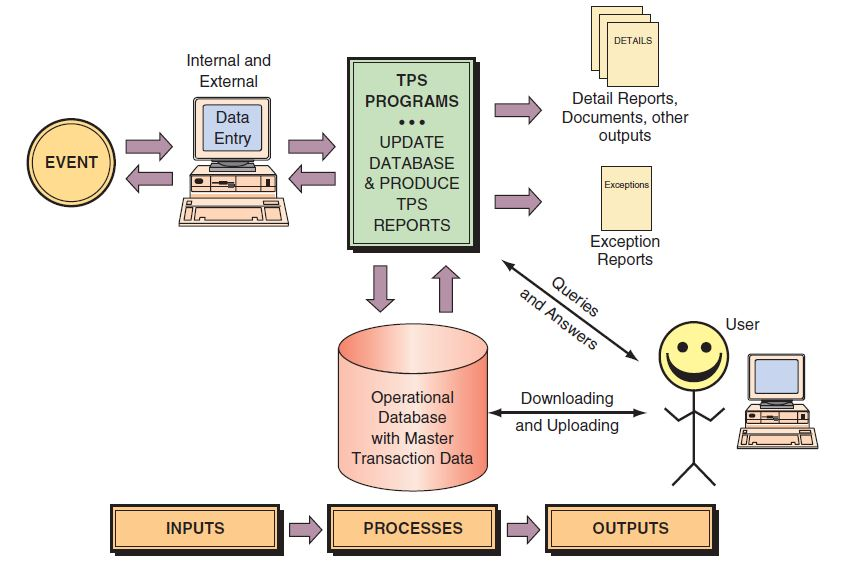
\includegraphics[scale=0.5]{F:/Skripsi/Dokumentasi_Skripsi/Gambar/Teori/tps.JPG}
		{\caption{Alur informasi pada proses transaksi} \cite{Turban:2001}}
	\label{fig:tps}
\end{figure}

Gambar \hyperlink{tps}{2.1} menggambarkan alur dari informasi pada proses transaksi yang akan dijelaskan sebagai berikut : 
\begin{enumerate}
	\item Sistem mencatat semua data yang dibutuhkan dari sebuah kejadian.
	\item Data kemudian disimpan ke dalam \textit{database}, apabila data tersebut belum terdapat pada \textit{database} maka akan dilakukan operasi \textit{insert} \textit{record} baru, sementara apabila data tersebut sudah dimiliki oleh \textit{database} maka akan dilakukan operasi \textit{update} untuk memperbaharui informasi pada \textit{record} yang sudah ada tersebut dengan informasi dari data baru.
	\item Apabila \textit{record} pada \textit{database} sudah berhasil ditambahkan/diperbaharui, program dapat menghasilkan laporan maupun dokumen yang dapat digunakan oleh pihak organisasi maupun dapat diakses oleh pihak luar.
\end{enumerate}

\textbf{Karakteristik TPS}\\
\label{sec:karakteristik_tps}

Berikut ini akan dijelaskan karakteristik dari TPS, antara lain \cite{Turban:2001} : 
\begin{enumerate}
	\item Volume data yang diproses sangat besar.
	\item Sumber data umumnya berasal dari dalam perusahaan dan keluaran yang dihasilkan dimaksudkan untuk pihak dalam perusahaan.
	\item Pemrosesan informasi dilakukan secara teratur. Misal harian, mingguan, dan sebagainya.
	\item Dibutuhkan kapasitas penyimpan (basis data) yang besar.
	\item Dibutuhkan kecepatan pemrosesan yang tinggi karena volume data yang diolah juga besar.
	\item Umumnya sistem memantau dan mengumpulkan data yang telah di-\textit{input} sebelumnya.
	\item Jenis data masukan dan keluaran sudah terstruktur. Karena data yang diproses cukup stabil, data diformat dalam suatu standar.
	\item Level kerincian yang tinggi terutama pada masukan tetapi seringkali juga pada keluaran.
	\item Komputasi tidak rumit (menggunakan operasi matematika sederhana atau operasi statistik).
	\item Dibutuhkan tingkat akurasi, integrasi dan keamanan data yang tinggi.
	\item Dibutuhkan tingkat keandalan yang tinggi.
	\item Pengaturan terhadap permintaan merupakan suatu hal wajib. TPS memungkinkan pengguna untuk melakukan \textit{query} terhadap basis data.
\end{enumerate}

\textbf{Contoh Aplikasi TPS}\\
\label{sec:contoh_aplikasi _tps}
Berikut ini akan dijelaskan aplikasi-aplikasi apa saja yang memanfaatkan sistem informasi berbentuk TPS berdasarkan fungsinya, yaitu \cite{Laudon:1996} :
\begin{enumerate}
	\item Sistem pemasaran (\textit{Sales})
	\item Sistem produksi (\textit{Manufacturing})
	\item Sistem akuntansi (\textit{Finance})
	\item Sistem ketenaga kerjaan (\textit{HR})
	\item Lain-lain (contoh : universitas)
\end{enumerate}

\subsection{\textit{Office Automation System} (OAS)}
\label{sec:oas}
\textit{Office Automation System} (OAS) adalah aplikasi yang didesain untuk meningkatkan produktivitas pegawai di kantor dengan mendukung koordinasi dan komunikasi antar pegawai \cite{Laudon:1996}. OAS digunakan untuk meningkatkan aliran pekerjaan dan komunikasi antar sesama pegawai, tidak peduli apakah pekerja tadi berada di satu lokasi yang sama ataupun tidak sehingga tingkat produktivitas pegawai dapat meningkat.

\textbf{Dampak dari Otomatisasi}\\
Otomatisasi proses dapat membawa dampak positif pada organisasi yang menerapkannya. Dampak dari otomatisasi terbagi menjadi 3 tingkatan yaitu \cite{Susan:1982}: 
\begin{enumerate}
	\item \textit{Innovative}\\
	Tingkat ini merupakan tahap awal dari otomatisasi. Pada level ini organisasi mulai menerapkan metode baru, penggunaan \textit{tools} dan teknik dalam pengerjaan beberapa tugasnya. Dampak otomatisasi pada level ini ditandai dengan tumbuhnya dan berkembangannya sektor bisnis.
	\item \textit{Rective}\\
	Tingkat ini organisasi mulai meningkatkan dukungan dan fasilitas untuk para manajer dan pegawai, kontorl sistem yang lebih baik dari sebelumnya dan semakin mudahnya mengakses suatu informasi yang akurat. Dampaknya produktivitas pegawai akan meningkat.
	\item \textit{Routine}\\
	Tingkat ini merupakan level teratas dari otomatisasi proses. Pada level ini hampir semua tugas yang ada pada organisasi sudah sebagian besar diotomatisasi. Dampaknya akan terasa pada berkurangnya biaya produksi dan peningkatan pada muatan pekerjaan dari staf pendukung.
\end{enumerate}
 
\section{\LaTeX}
\label{sec:latex}
\LaTeX adalah sebuah bahasa markup untuk sistem penulisan dokumen yang dikembangkan oleh Leslie B. Lamport dan dirilis pada tahun 1985 \cite{Lamport:1994}. \LaTeX memiliki filosofi WYMIWYG (\textit{What You Mean Is What You Get}) yang berarti sesuatu yang akan kita tulis akan ditulis berdasarkan arti dari hal tersebut. Oleh karena itu, untuk menambahkan suatu perintah pada dokumen yang sedang kita tulis perlu menambahkan suatu \textit{command}. \textit{Command} adalah kata spesial yang menentukan suatu sifat pada \LaTeX. Hampir semua \textit{command} pada \LaTeX selalu diawali dengan tanda '\textbackslash' dan beberapa \textit{command} memiliki \textit{parameter}. \textit{Parameter} diawali dengan tanda kurung kurawal buka dan diakhiri denga kurung kurawal tutup(\{\}). \textit{File} \LaTeX memiliki ekstensi .tex.  

Untuk menulis dokumen pada \LaTeX dibutuhkan beberapa \textit{command} yang wajib ada dalam sebuah dokumen, yaitu \cite{Lamport:1994} : 
\begin{enumerate}
	\item \texttt{\string\documentclass[option]\{class\}}\\
	Digunakan untuk menentukan jenis dokumen dan \textit{layout} dokumen. Bagian \textit{option} dapat dikosongkan atau dapat digunakan untuk menyimpan pilihan pengaturan \textit{layouting}. Pada bagian \textit{class} digunakan untuk menentukan tipe dokumen yang akan dibuat.
	\item \texttt{\string\usepackage\{package name\}}\\
	Digunakan untuk menambahkan sebuah \textit{package} baru untuk mendukung pembuatan dokumen. Package adalah sebuah pengaturan yang berisi sekumpulan \textit{command} dan pengaturan yang akan digunakan untuk mengatur keseluruhan isi dokumen. \textit{Package name} diisi dengan nama \textit{package} yang akan digunakan.
	\item \texttt{\string\title\{\}}\\
	Digunakan untuk menapilkan halaman judul. Biasanya halaman judul akan memuat judul dokumen, nama pengarang dan tanggal pembuatan dokumen. Nama pengarang dan tanggal pembuatan dapat ditampilkan dengan menambahkan perintah \texttt{\string\author\{nama\}} dan \texttt{\string\date\{tanggal\}}
	\item \texttt{\string\begin\{document\}}...\texttt{\string\end\{document\}}\\
	Digunakan untuk mengawali dan mengakhiri isi dokumen.
\end{enumerate}

\subsection{Mailmerge}
\label{sec:mailmerge}
\textit{Mailmerge} adalah salah satu \textit{package} yang disediakan oleh \LaTeX yang berupa antar muka untuk pembuatan surat atau dokumen. \textit{Mailmerge} memilik 2 komponen utama yaitu \textit{repeated text} yaitu sejumlah tulisan dalam dokumen tersebut yang ditulis sama persis berulang kali pada setiap pengulangan, dan \textit{command} yang dapat diganti-ganti dengan suatu nilai tertentu pada setiap pengulangan \cite{Frasson:2009} .\

Untuk menggunakan \textit{package mailmerge}, ada beberapa \textit{command} yang perlu ditambahkan seperti \cite{Frasson:2009} :
\begin{enumerate}
	\item \texttt{\string\mailfields}\\
	Digunakan untuk menyatakan nama \textit{field} yang akan digunakan. Nama \textit{field} disimpan di dalam \textit{parameter} \texttt{\string\mailfields}. Urutan nama \textit{field} yang dideklarasikan akan berpengaruh pada \texttt{\string\mailentry}. Nama \textit{field} akan menjadi \textit{parameter} bagi \textit{command} \texttt{\string\field}.
	\item \texttt{\string\mailrepeat}\\
	Digunakan untuk menentukan teks mana saja yag diulang setiap kali pengulangan. Teks yang akan diulang maupun \textit{command} \texttt{\string\field} akan menjadi parameter bagi \texttt{\string\mailrepeat}, namun isi dari \textit{command} \texttt{\string\field} akan berubah pada setiap kali pengulangan sesuai dengan data pada \textit{entry}.
	\item \texttt{\string\mailentry}\\
	Digunakan untuk penampungan nilai sebelum dimasukkan sebagai \textit{parameter} \textit{command} \texttt{\string\field}.
\end{enumerate}
	Berikut ini adalah urutan tata letak setiap \textit{command} untuk pembuatan \textit{mailmerge} :
	\begin{lstlisting}[language=tex,basicstyle=\tiny,caption=Contoh pembuatan \textit{mailmerge}]
	\documentclass[12pt]{letter}
    \usepackage{ifthen,mailmerge}

    % \ifequal{A}{B}{what if A=B}{what if A<>B}
    \newcommand{\ifequal}[2]{\ifthenelse{\equal{#1}{#2}}}

    \mailfields{name,friends,drives}

    \mailrepeat{\section*{\field{name}'s profile}

       \field{name} has
       \ifequal{\field{friends}}{}
         {no friends}
         {\field{friends} as friends}.
       \ifequal{\field{drives}}{yes}{Drives.}{Doesn't drive.}

    (entry \entrynumber\ of \numberofentries)

    % \newpage optional
    }

    \mailentry{John,{Bart and Robert},yes}
    \mailentry{Sara,{Jean, Phillip and Maria},no}
    \mailentry{Edward,,yes}
 \end{lstlisting}
 
\section{Laravel}
\label{sec:laravel}
Laravel adalah \textit{framework web} berbasis php yang bersifat \textit{open-source} yang dikembangkan oleh Taylor Otwell pada Juni 2011\cite{surguy:2013}. Laravel menerapkan pola arsitektur \textit{Model-View-Controller} (MVC) dimana \textit{layer} memiliki fungsi yang berbeda-beda.

\subsection{Komponen Utama Laravel}
\label{sec:komponen_utama_laravel}
Laravel memiliki beberapa \textit{file} yang menjadi komponen utama yang perlu diperhatikan. \textit{File-file} tersebut yaitu\cite{laravel:2016} :
\begin{itemize}
	\item \textit{Model}\\
	\textit{Model} merupakan bagian yang menghubungkan antara aplikasi dengan \textit{database}.
	\item \textit{View}\\
	\textit{View} merupakan bagian yang bertugas menampilkan \textit{file} tampilan ke pengguna.  
	\item \textit{Controller}\\
	\textit{Controller} bertugas menjalankan proses lojik dan juga menerima \textit{input request} dari \textit{view}.
	\item \textit{Route}\\
	\textit{Route} bertugas mengatur pemetaan jalur \textit{request} dari \textit{view} ke \textit{controller}.  
\end{itemize}